% Options for packages loaded elsewhere
\PassOptionsToPackage{unicode}{hyperref}
\PassOptionsToPackage{hyphens}{url}
\documentclass[
]{article}
\usepackage{xcolor}
\usepackage[margin=1in]{geometry}
\usepackage{amsmath,amssymb}
\setcounter{secnumdepth}{-\maxdimen} % remove section numbering
\usepackage{iftex}
\ifPDFTeX
  \usepackage[T1]{fontenc}
  \usepackage[utf8]{inputenc}
  \usepackage{textcomp} % provide euro and other symbols
\else % if luatex or xetex
  \usepackage{unicode-math} % this also loads fontspec
  \defaultfontfeatures{Scale=MatchLowercase}
  \defaultfontfeatures[\rmfamily]{Ligatures=TeX,Scale=1}
\fi
\usepackage{lmodern}
\ifPDFTeX\else
  % xetex/luatex font selection
\fi
% Use upquote if available, for straight quotes in verbatim environments
\IfFileExists{upquote.sty}{\usepackage{upquote}}{}
\IfFileExists{microtype.sty}{% use microtype if available
  \usepackage[]{microtype}
  \UseMicrotypeSet[protrusion]{basicmath} % disable protrusion for tt fonts
}{}
\makeatletter
\@ifundefined{KOMAClassName}{% if non-KOMA class
  \IfFileExists{parskip.sty}{%
    \usepackage{parskip}
  }{% else
    \setlength{\parindent}{0pt}
    \setlength{\parskip}{6pt plus 2pt minus 1pt}}
}{% if KOMA class
  \KOMAoptions{parskip=half}}
\makeatother
\usepackage{graphicx}
\makeatletter
\newsavebox\pandoc@box
\newcommand*\pandocbounded[1]{% scales image to fit in text height/width
  \sbox\pandoc@box{#1}%
  \Gscale@div\@tempa{\textheight}{\dimexpr\ht\pandoc@box+\dp\pandoc@box\relax}%
  \Gscale@div\@tempb{\linewidth}{\wd\pandoc@box}%
  \ifdim\@tempb\p@<\@tempa\p@\let\@tempa\@tempb\fi% select the smaller of both
  \ifdim\@tempa\p@<\p@\scalebox{\@tempa}{\usebox\pandoc@box}%
  \else\usebox{\pandoc@box}%
  \fi%
}
% Set default figure placement to htbp
\def\fps@figure{htbp}
\makeatother
\setlength{\emergencystretch}{3em} % prevent overfull lines
\providecommand{\tightlist}{%
  \setlength{\itemsep}{0pt}\setlength{\parskip}{0pt}}
\usepackage{pdflscape}
\usepackage{afterpage}
\usepackage{bookmark}
\IfFileExists{xurl.sty}{\usepackage{xurl}}{} % add URL line breaks if available
\urlstyle{same}
\hypersetup{
  pdftitle={Supplementary Figures},
  hidelinks,
  pdfcreator={LaTeX via pandoc}}

\title{Supplementary Figures}
\author{}
\date{\vspace{-2.5em}}

\begin{document}
\maketitle

\newpage

\textbf{Fig. S1} \textbar{} \emph{tbd} Map of 35 islands surveyed by
CREP across the tropical Pacific.

\begin{landscape}


\begin{center}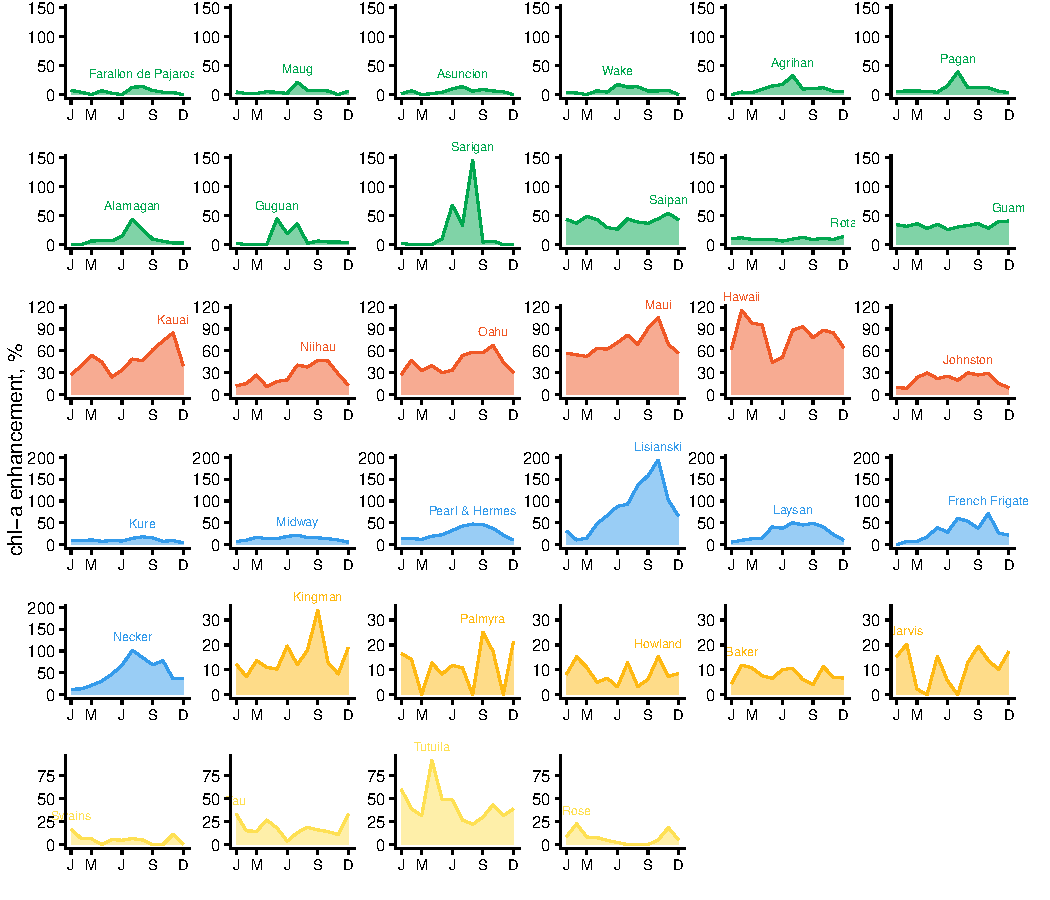
\includegraphics[width=0.75\linewidth]{fig/FigureSX_IME} \end{center}
\textbf{Fig. S2} | Seasonal variation in IME strength at each island. Lines are mean-monthly chl-a enhancement from January to December, ordered and coloured by island group.
\end{landscape}
\newpage

\begin{center}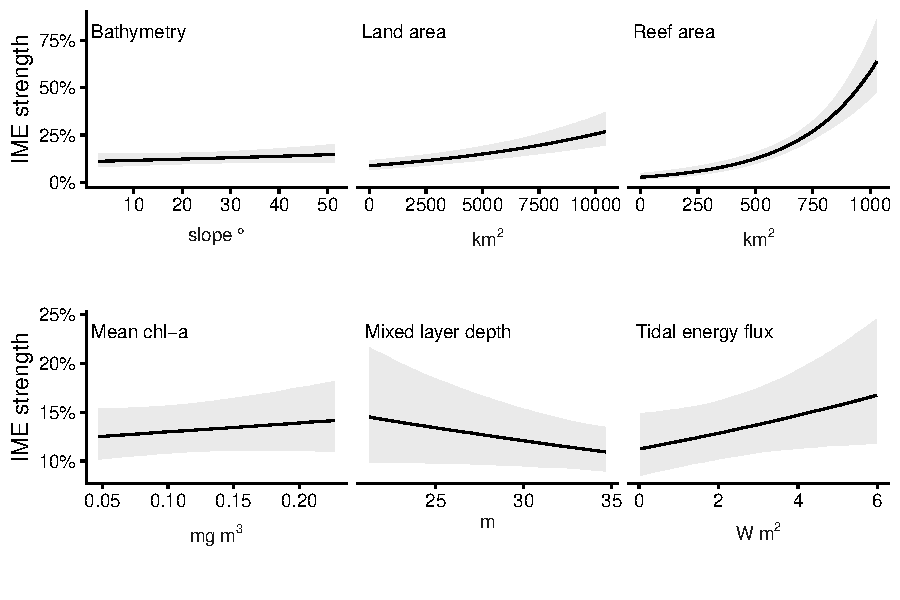
\includegraphics[width=0.85\linewidth]{fig/FigureSX_IME_pred} \end{center}

\textbf{Fig. S3} \textbar{} Spatial effects on chl-a enhancement for
geomorphic features (top) and average oceanographic conditions (bottom)
Lines are median posterior predictions (± 95\% certainty intervals).
Note different y-axis values between static and dynamic covariates.
\newpage

\begin{center}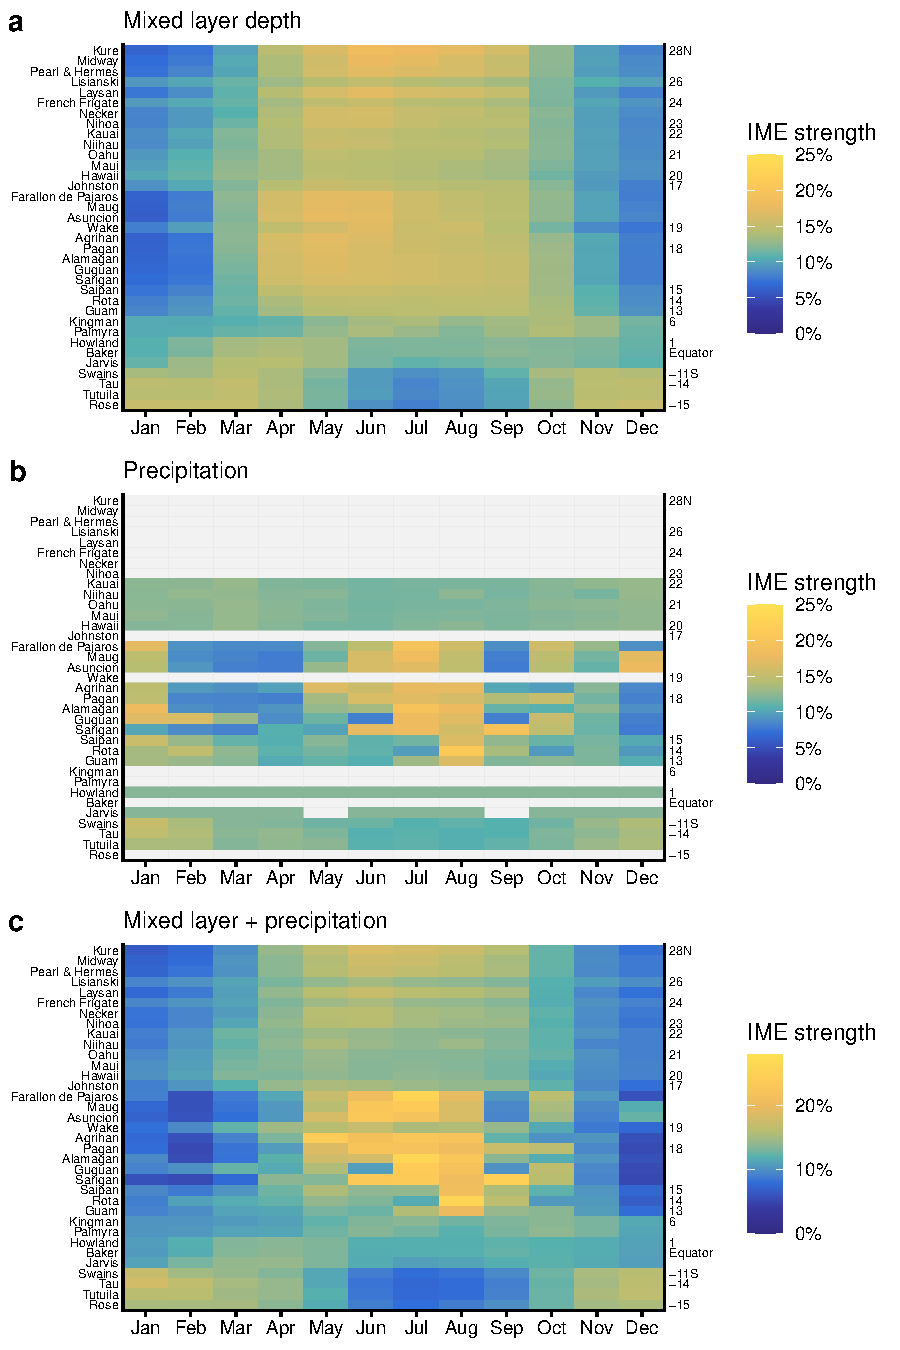
\includegraphics[width=0.85\linewidth]{fig/FigureSX_IME_seasonal_pred} \end{center}

\textbf{Fig. S4} \textbar{} Heatmap of seasonal effects on chl-a
enhancement for a mixed layer depth, b precipitation and c both
covariates combined. Islands with less than 1 mm monthly rainfall are
shown in grey. All values are median posterior predictions excluding
effects of other covariates. \newpage

\begin{landscape}


\begin{center}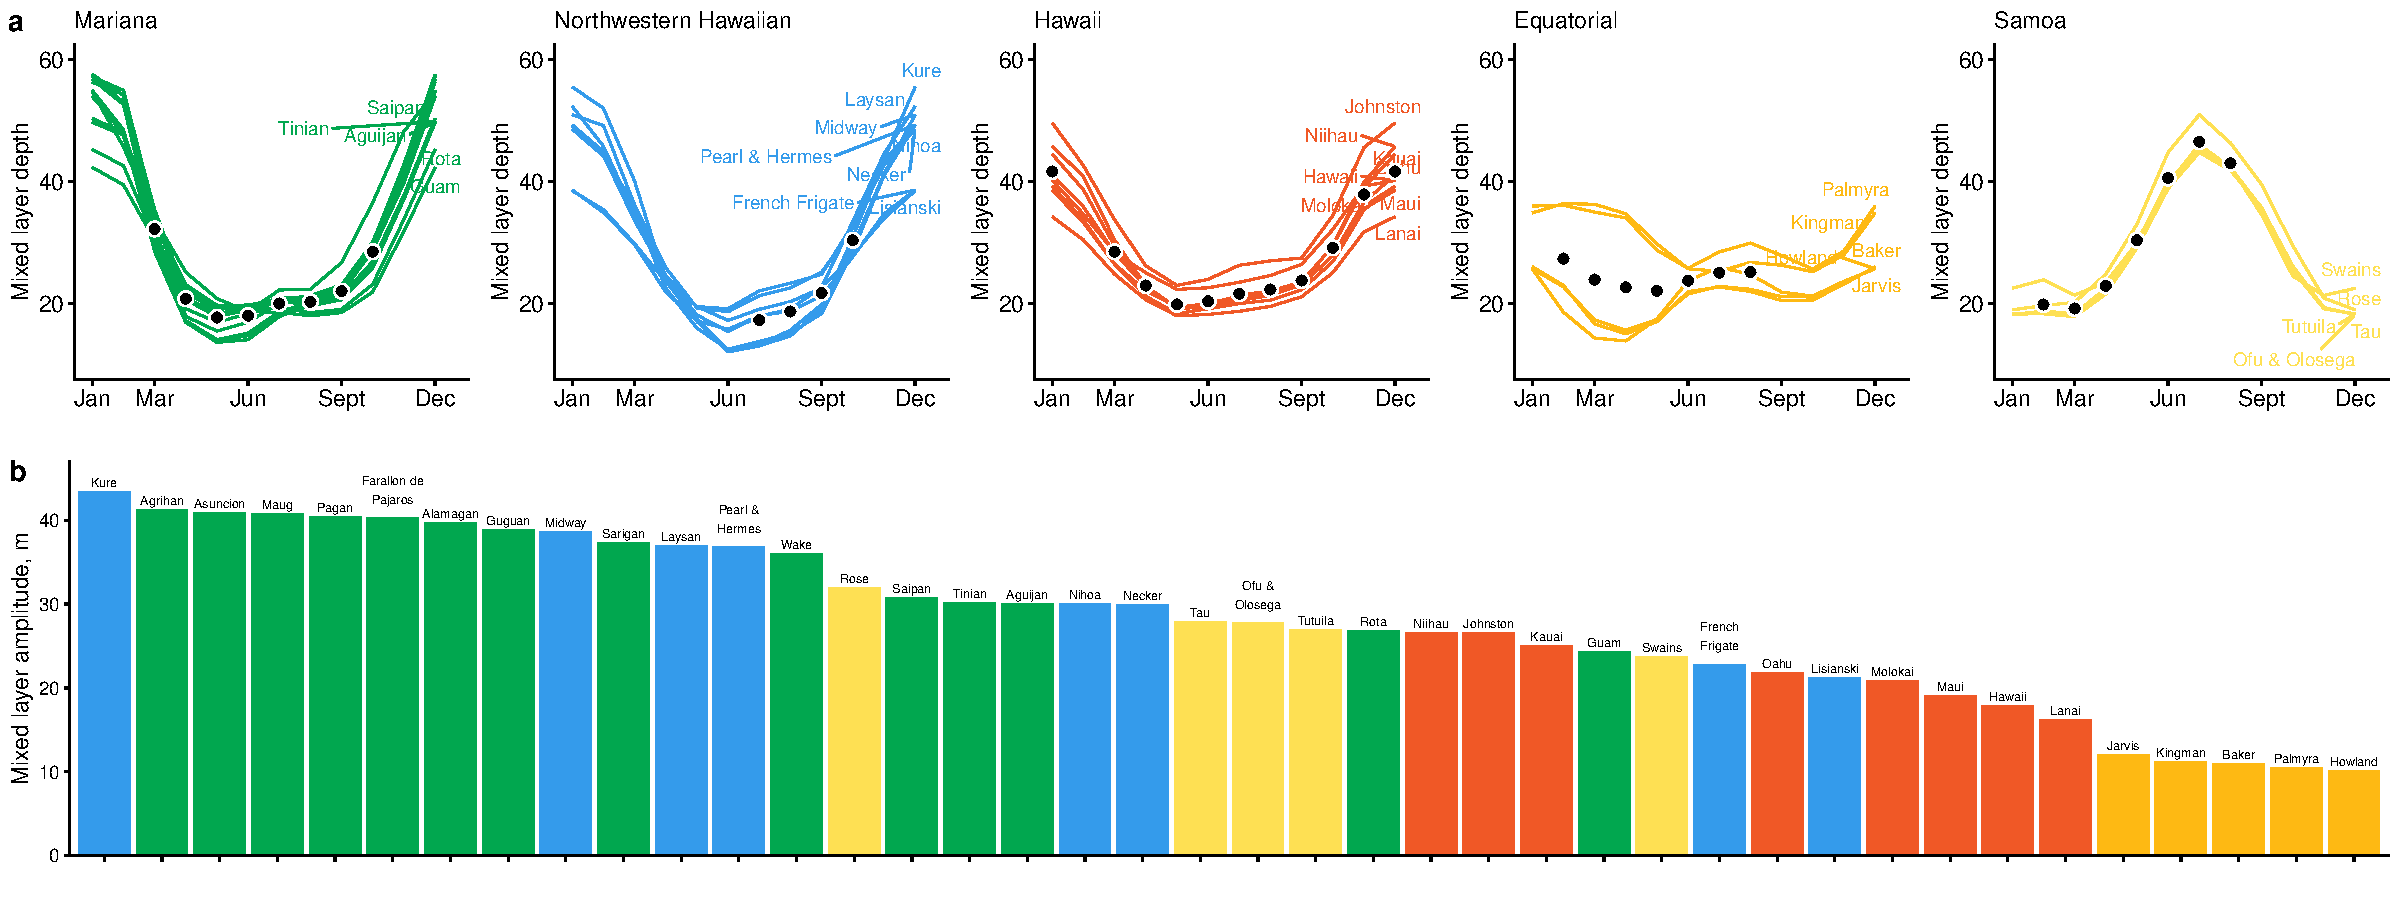
\includegraphics[width=0.95\linewidth]{fig/FigureSX_MLD_amp} \end{center}
\textbf{Fig. S5} | Seasonal variability in the mixed layer depth at each island. In a, lines are predicted mixed layer depth at each island from a General Additive Model with smoothers for time and month (cyclic), overlaid with points indicating timing of coral reef fish surveys.
\end{landscape}
\newpage

\begin{center}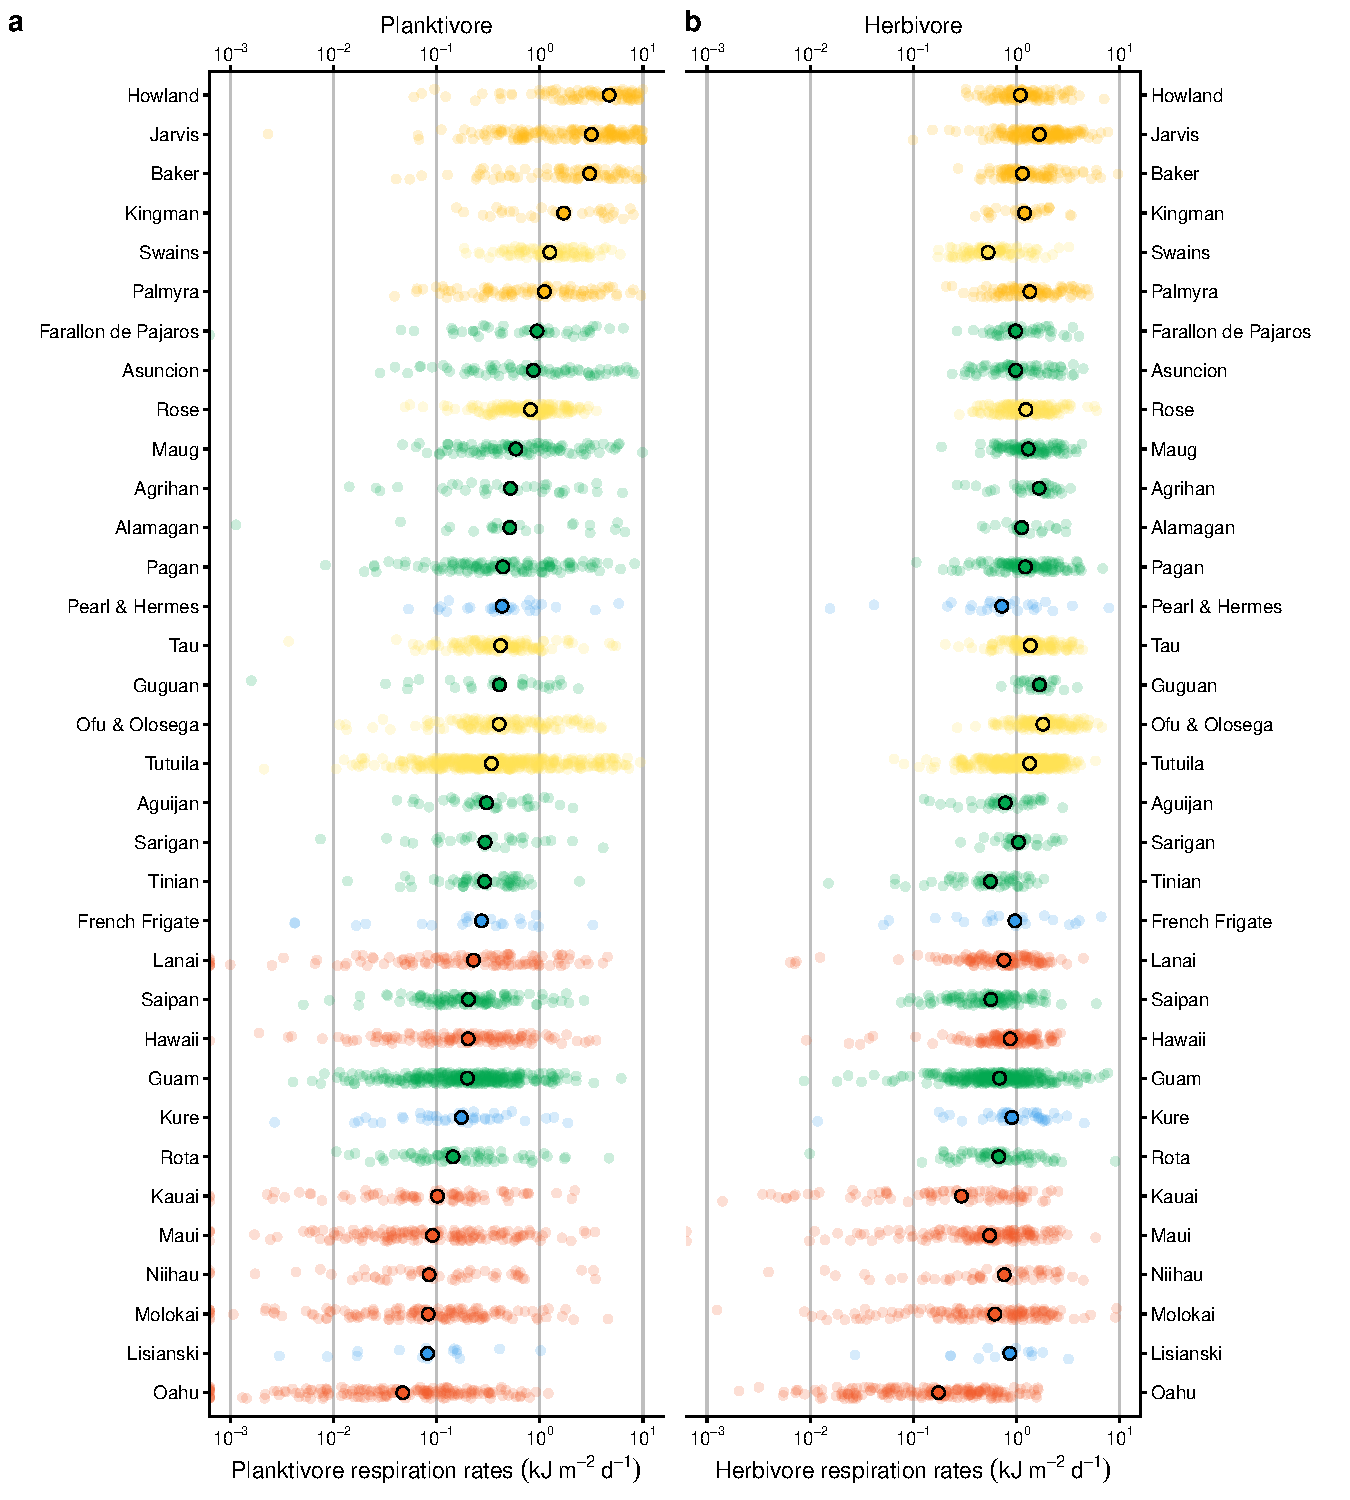
\includegraphics[width=0.95\linewidth,height=0.8\textheight]{fig/FigureSX_metab} \end{center}

\textbf{Fig. S6} \textbar{} Respiration rate of reef-associated
planktivores on coral reefs at 34 Pacific islands and atolls. Each point
is the median respiration at each island, with jitter showing unique
sites (n = 3,622). \newpage

\begin{landscape}


\begin{center}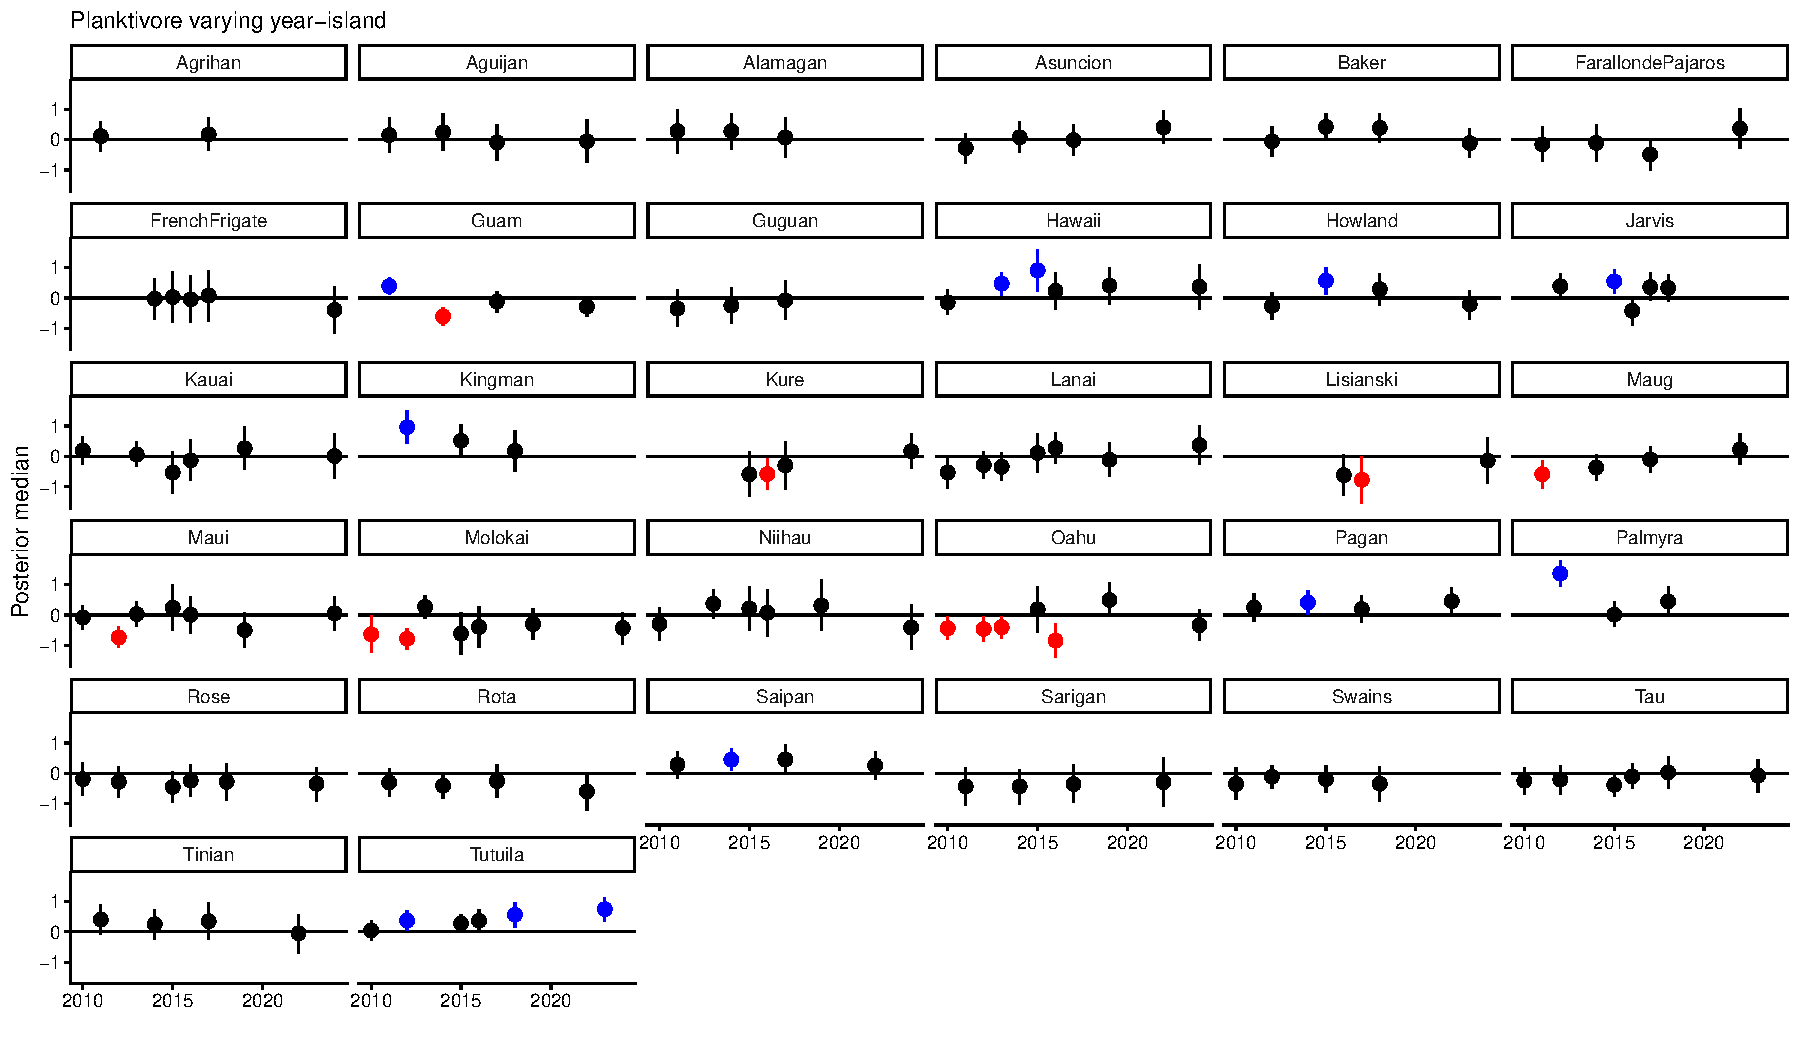
\includegraphics[width=0.95\linewidth,height=0.8\textheight]{fig/FigureSX_planktivore_time} \end{center}

\textbf{Fig. S7} | Effect of survey year on planktivore respiration rate. Points are posterior medians with 95\% certainty intervals, coloured when the posterior did not overlap zero (red = negative, blue = positive).
\newpage


\begin{center}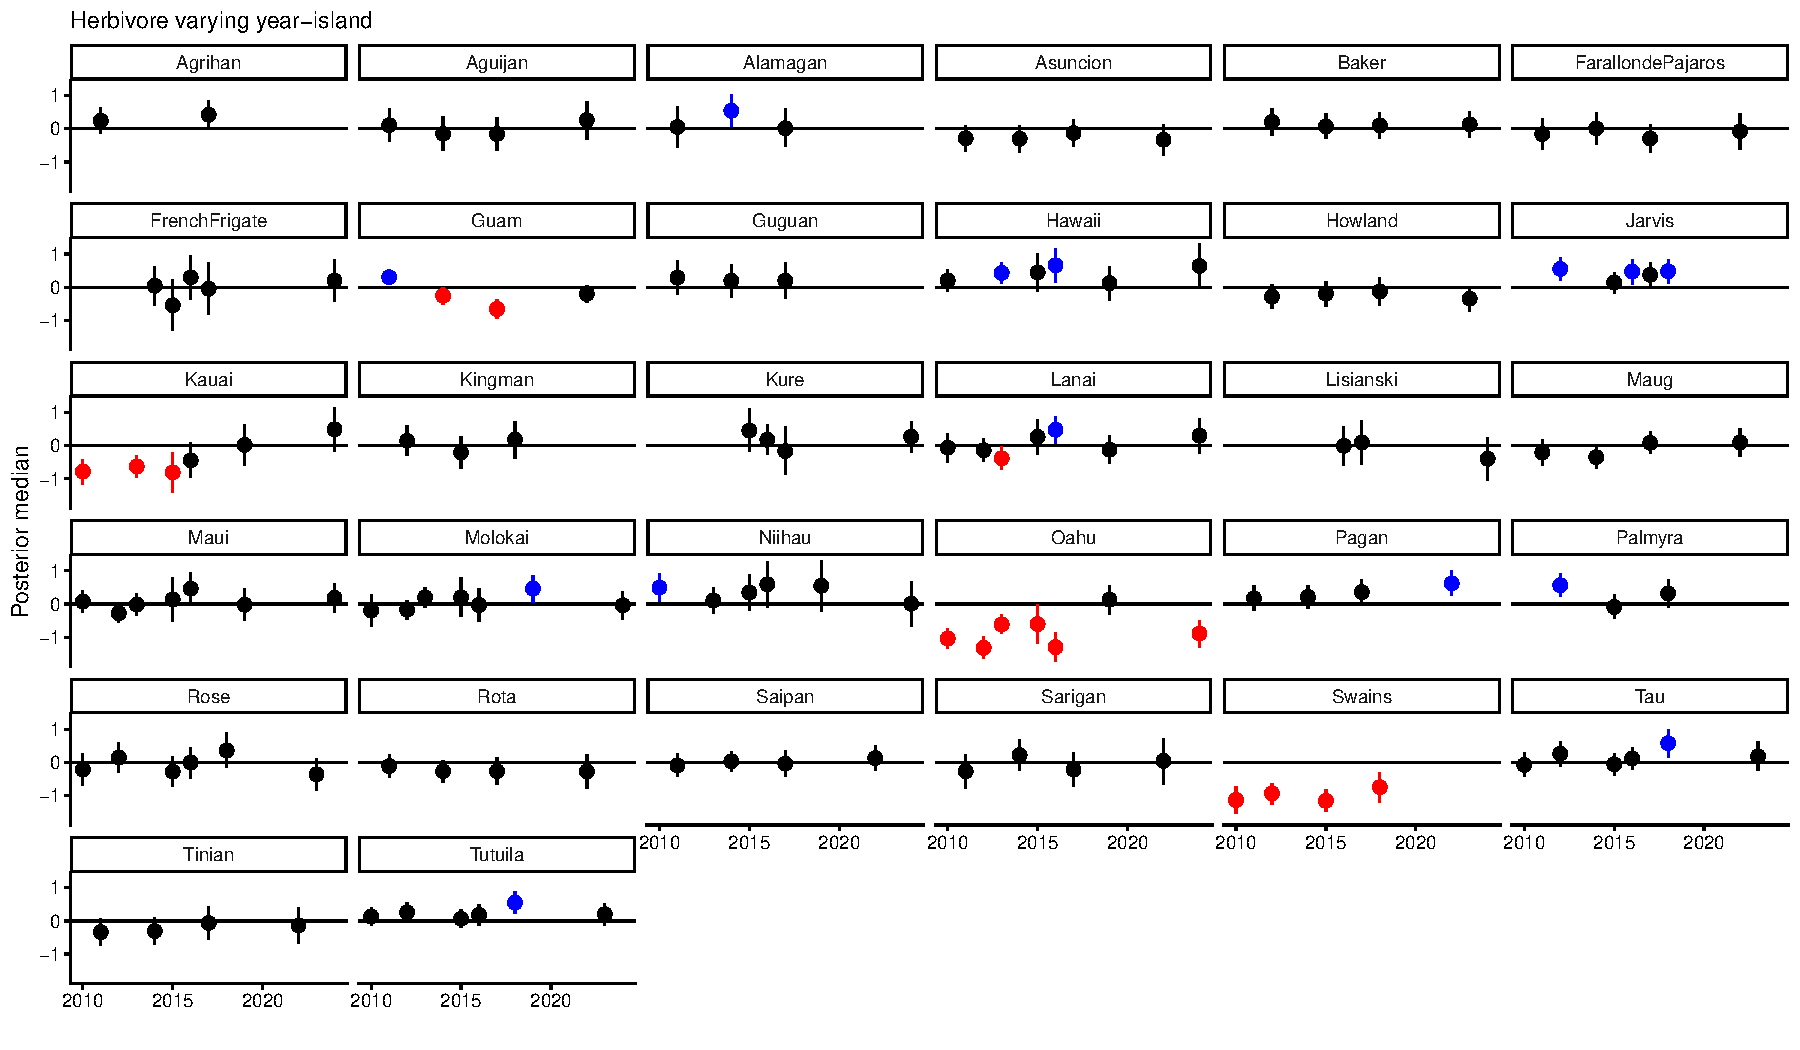
\includegraphics[width=0.95\linewidth]{fig/FigureSX_herbivore_time} \end{center}

\textbf{Fig. S8} | Effect of survey year on herbivore respiration rate. Points are posterior medians with 95\% certainty intervals, coloured when the posterior did not overlap zero (red = negative, blue = positive).
\newpage
\end{landscape}

\begin{center}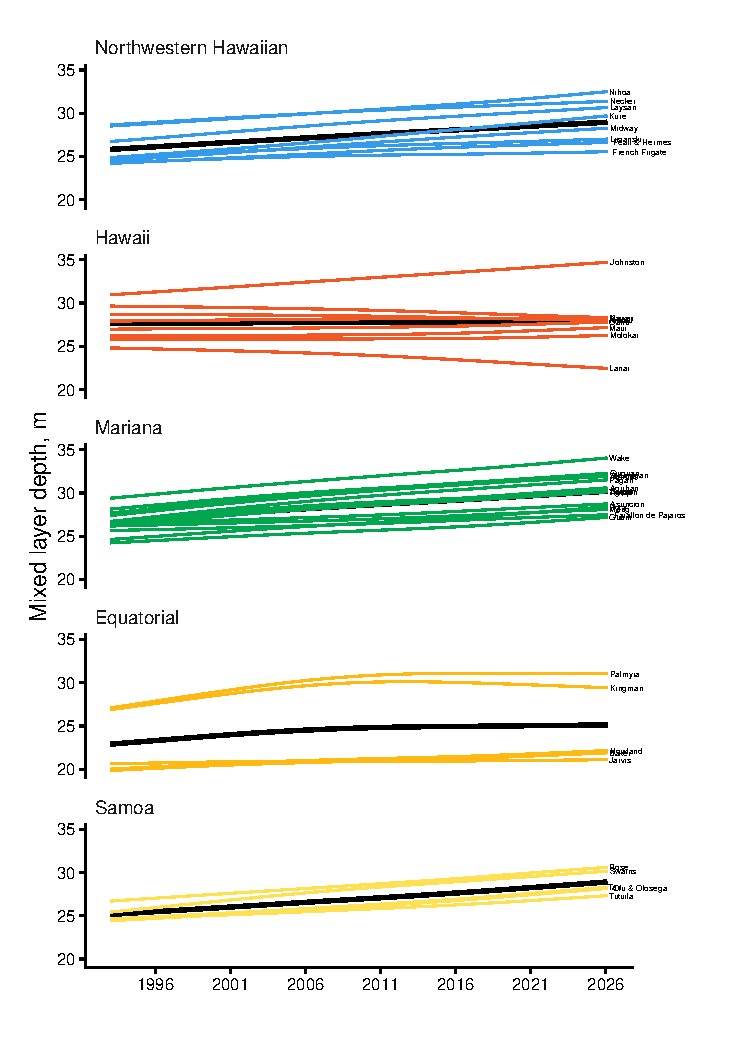
\includegraphics[height=0.85\textheight]{fig/FigureSX_MLD_time_obs} \end{center}

\textbf{Fig. S9} \textbar{} Island-level temporal trends in the mixed
layer depth layer from 1993-2026. Lines are mean predicted mixed layer,
accounting for monthly variability, from a generalised additive model,
for each region (black with 95\% CI filled by region) and overlaid with
mean island predictions (coloured lines).

\newpage

\begin{center}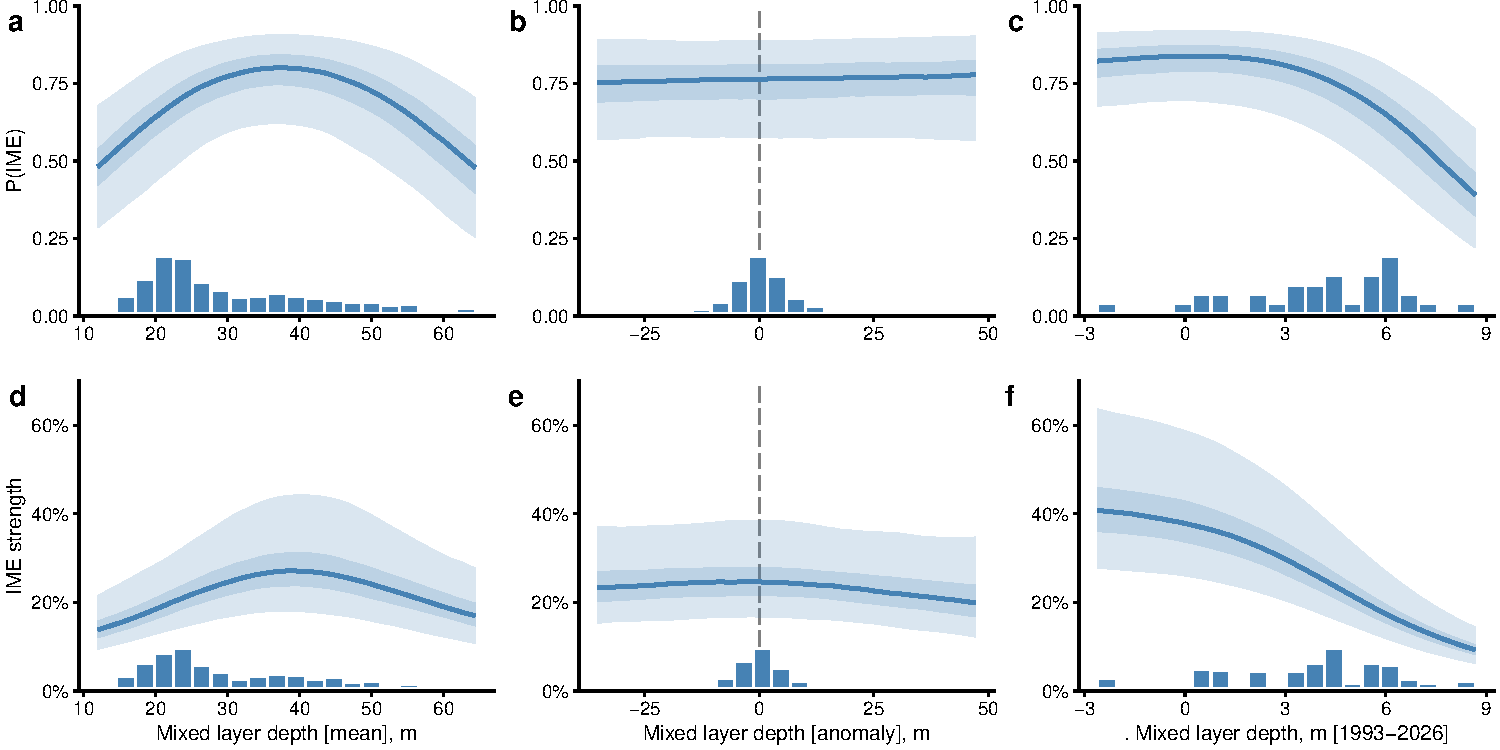
\includegraphics[width=0.85\linewidth]{fig/FigureSX_IME_time_covariates} \end{center}

\textbf{Fig. S10} \textbar{} Effects of mixed layer depth covariates on
IME dynamics from 1997-2025. a) Probability of detecting an IME and b)
IME strength (\%). Lines are median posterior estimates with 95\% and
50\% certainty intervals.

\newpage
\begin{landscape}


\begin{center}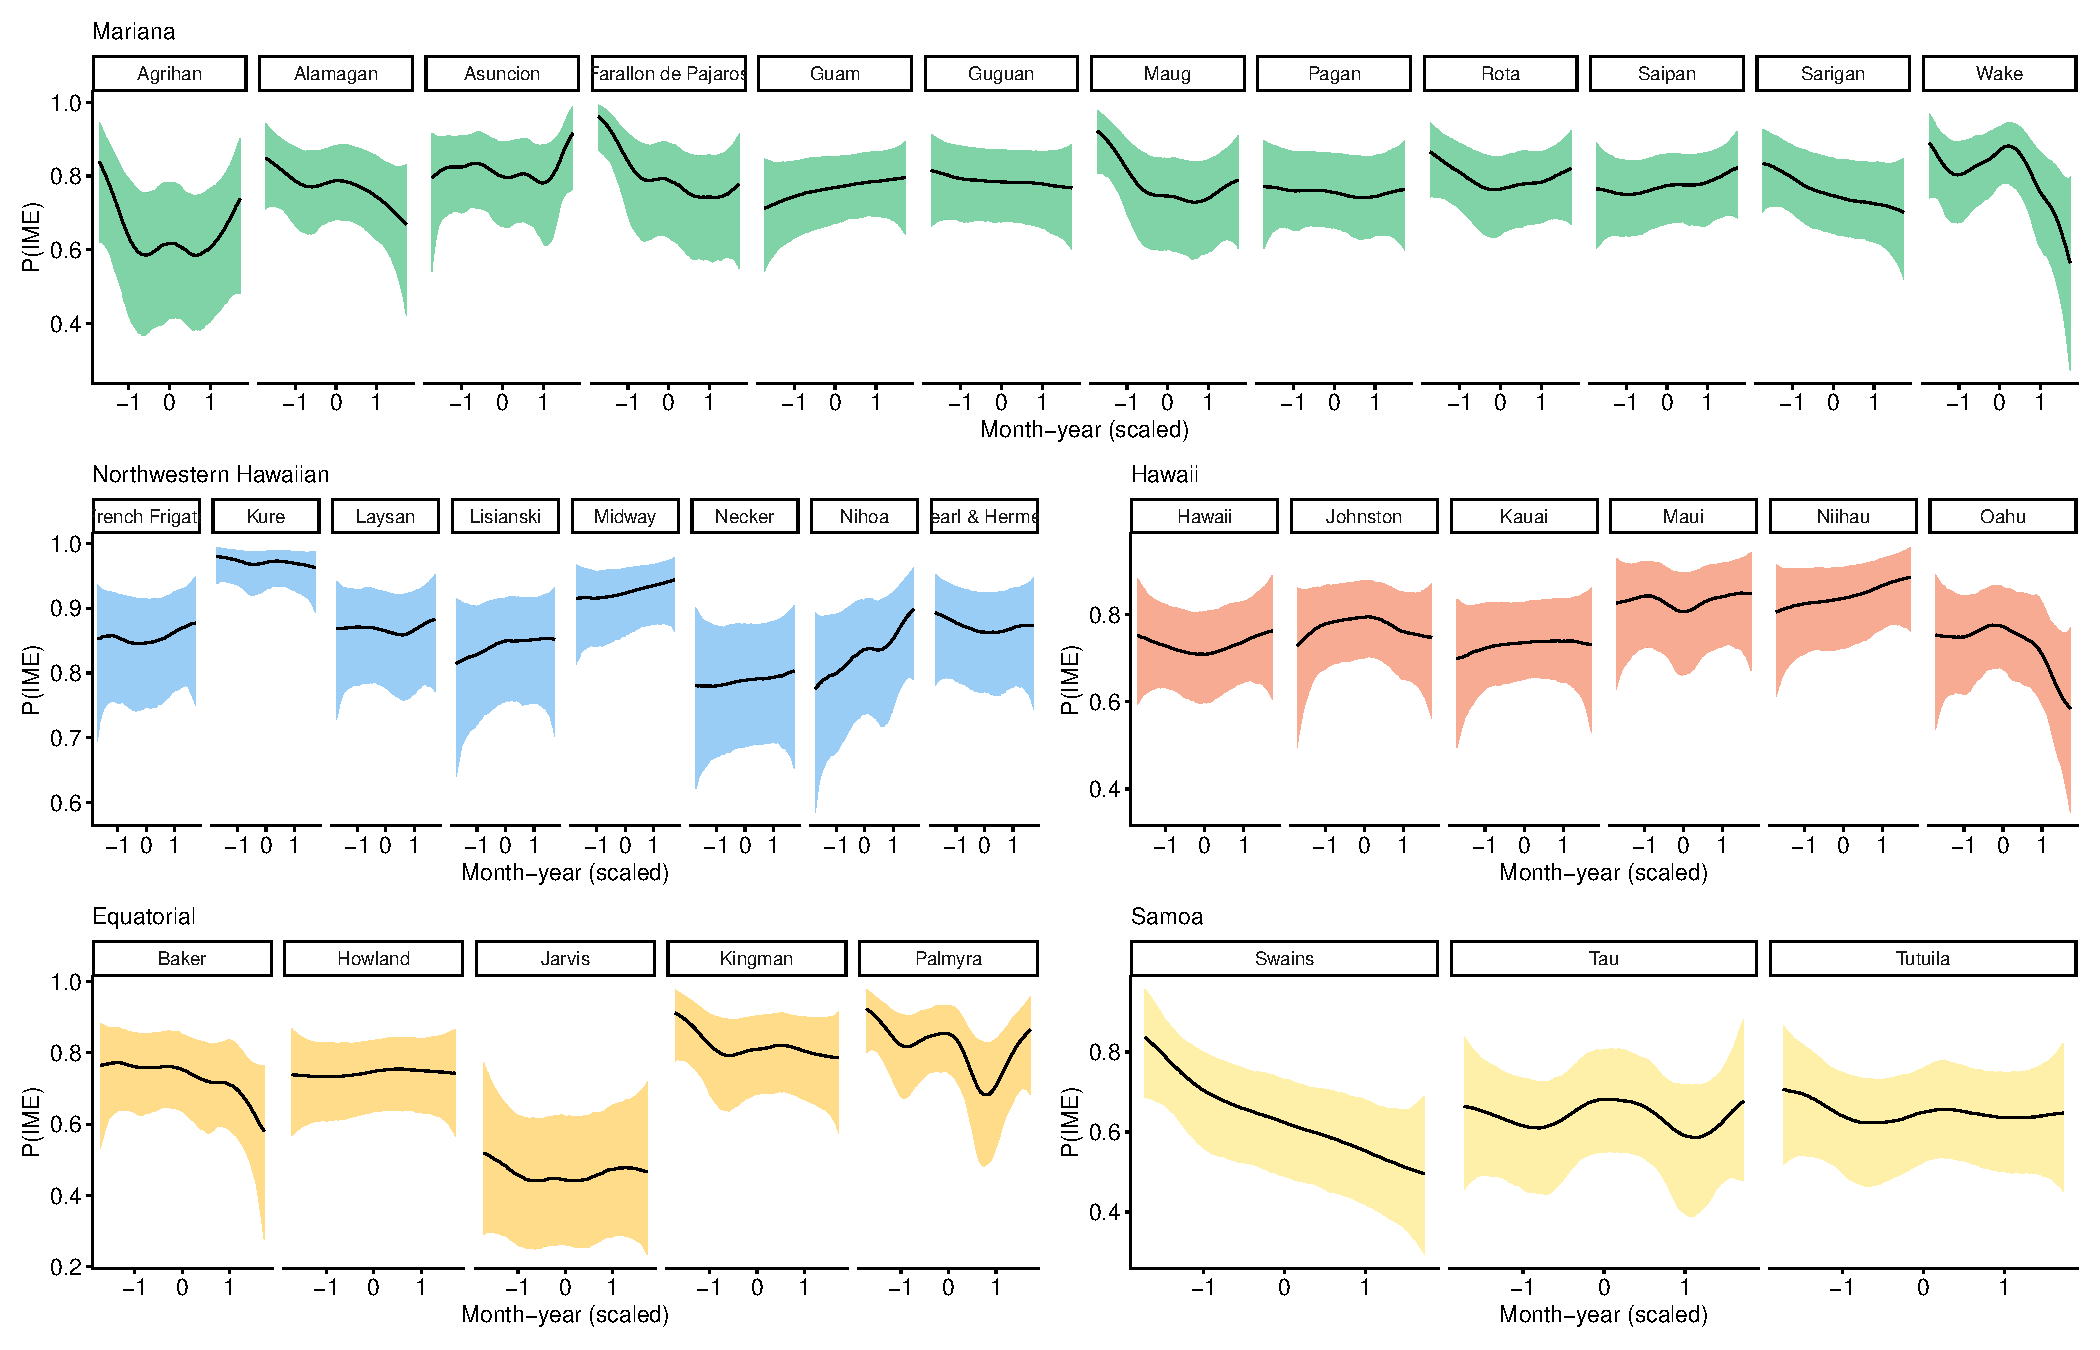
\includegraphics[width=0.95\linewidth]{fig/FigureSX_IME_temporalFullDetect} \end{center}

\textbf{Fig. S11} | Temporal change in the probability of IME occurrence at each island from 1997-2025. Lines are median posterior estimates with 95% and 50% certainty intervals, excluding effects of mixed layer covariates and month smoother.

\newpage


\begin{center}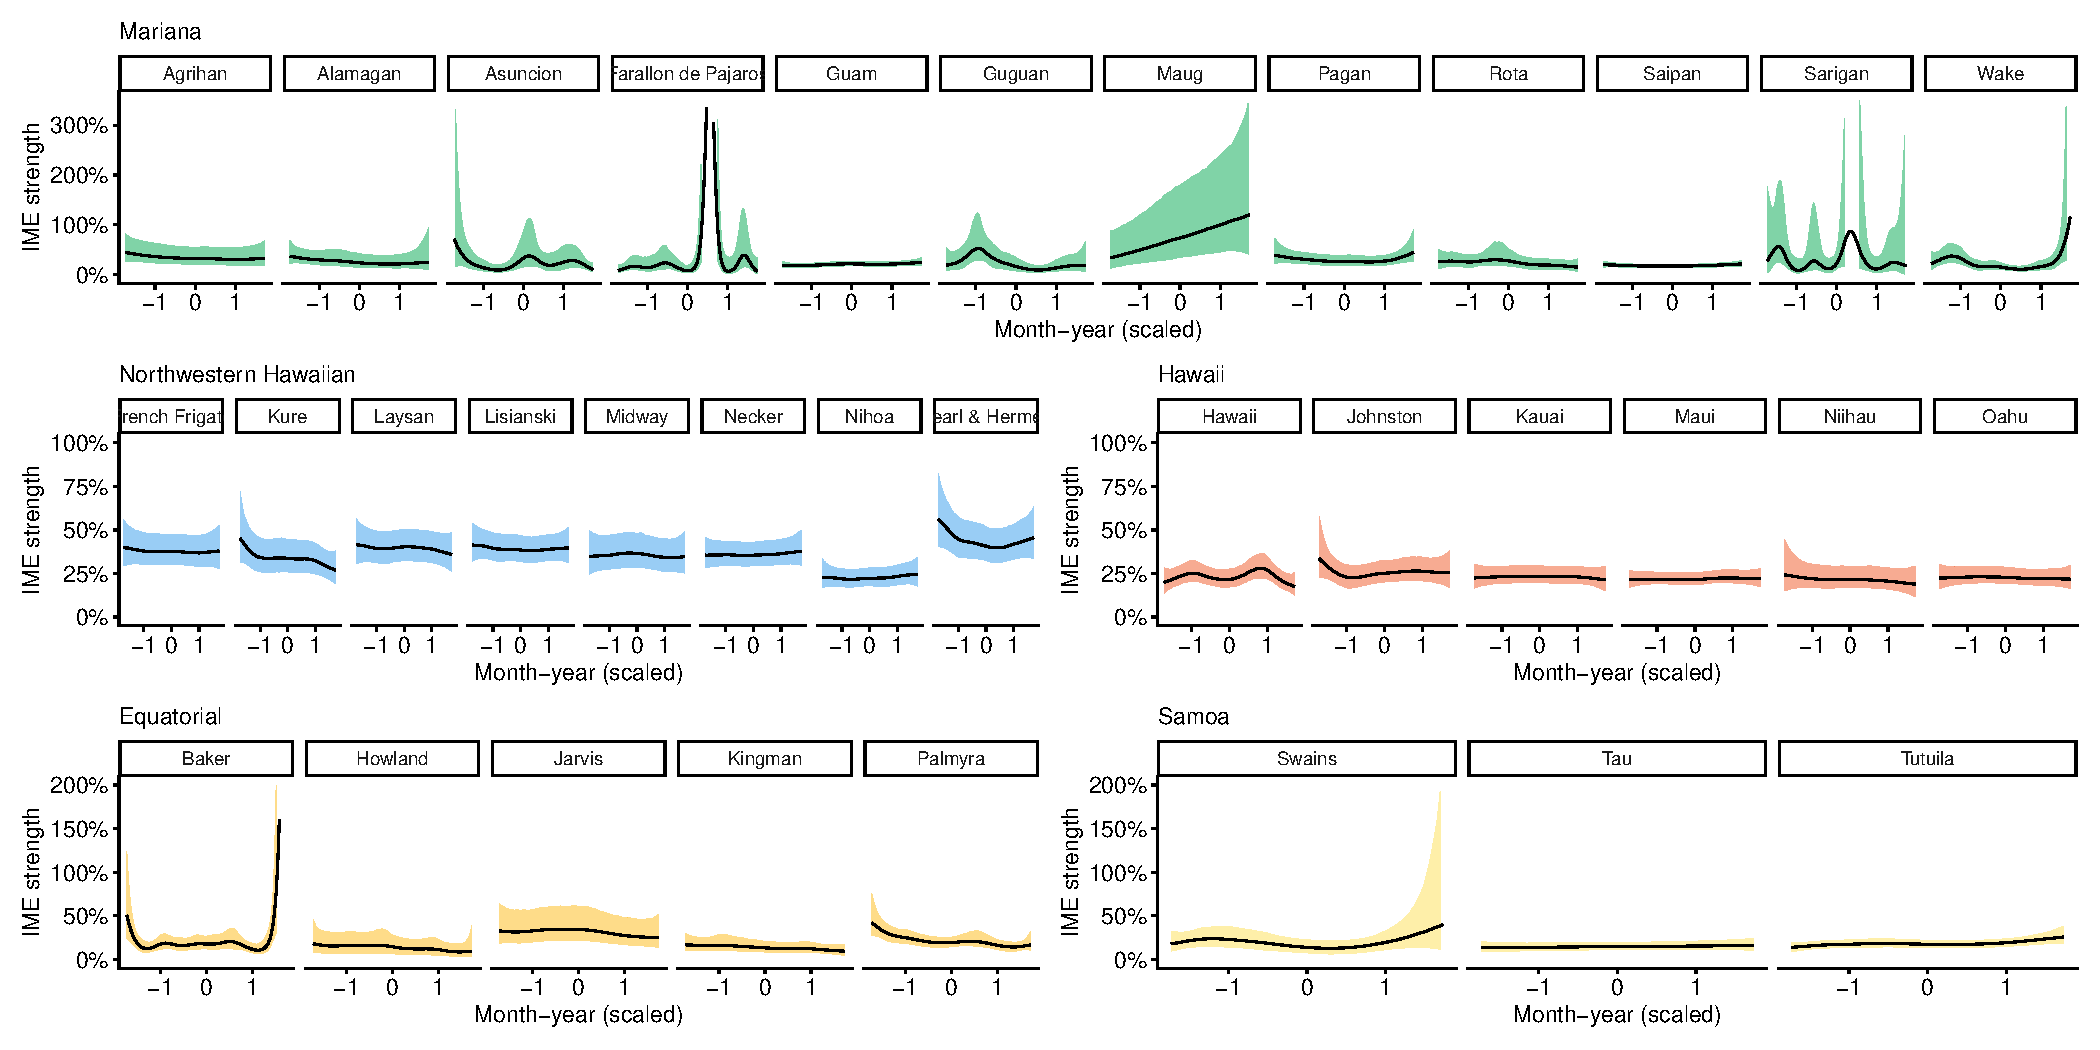
\includegraphics[width=0.95\linewidth]{fig/FigureSX_IME_temporalFullGamma} \end{center}

\textbf{Fig. S12} | Temporal change in the IME strength at each island from 1997-2025. Lines are median posterior estimates with 95% and 50% certainty intervals, excluding effects of mixed layer covariates and month smoother.

\end{landscape}

\end{document}
